% Options for packages loaded elsewhere
\PassOptionsToPackage{unicode}{hyperref}
\PassOptionsToPackage{hyphens}{url}
%
\documentclass[
]{article}
\author{}
\date{\vspace{-2.5em}}

\usepackage{amsmath,amssymb}
\usepackage{lmodern}
\usepackage{iftex}
\ifPDFTeX
  \usepackage[T1]{fontenc}
  \usepackage[utf8]{inputenc}
  \usepackage{textcomp} % provide euro and other symbols
\else % if luatex or xetex
  \usepackage{unicode-math}
  \defaultfontfeatures{Scale=MatchLowercase}
  \defaultfontfeatures[\rmfamily]{Ligatures=TeX,Scale=1}
\fi
% Use upquote if available, for straight quotes in verbatim environments
\IfFileExists{upquote.sty}{\usepackage{upquote}}{}
\IfFileExists{microtype.sty}{% use microtype if available
  \usepackage[]{microtype}
  \UseMicrotypeSet[protrusion]{basicmath} % disable protrusion for tt fonts
}{}
\makeatletter
\@ifundefined{KOMAClassName}{% if non-KOMA class
  \IfFileExists{parskip.sty}{%
    \usepackage{parskip}
  }{% else
    \setlength{\parindent}{0pt}
    \setlength{\parskip}{6pt plus 2pt minus 1pt}}
}{% if KOMA class
  \KOMAoptions{parskip=half}}
\makeatother
\usepackage{xcolor}
\IfFileExists{xurl.sty}{\usepackage{xurl}}{} % add URL line breaks if available
\IfFileExists{bookmark.sty}{\usepackage{bookmark}}{\usepackage{hyperref}}
\hypersetup{
  hidelinks,
  pdfcreator={LaTeX via pandoc}}
\urlstyle{same} % disable monospaced font for URLs
\usepackage[margin=1in]{geometry}
\usepackage{color}
\usepackage{fancyvrb}
\newcommand{\VerbBar}{|}
\newcommand{\VERB}{\Verb[commandchars=\\\{\}]}
\DefineVerbatimEnvironment{Highlighting}{Verbatim}{commandchars=\\\{\}}
% Add ',fontsize=\small' for more characters per line
\usepackage{framed}
\definecolor{shadecolor}{RGB}{248,248,248}
\newenvironment{Shaded}{\begin{snugshade}}{\end{snugshade}}
\newcommand{\AlertTok}[1]{\textcolor[rgb]{0.94,0.16,0.16}{#1}}
\newcommand{\AnnotationTok}[1]{\textcolor[rgb]{0.56,0.35,0.01}{\textbf{\textit{#1}}}}
\newcommand{\AttributeTok}[1]{\textcolor[rgb]{0.77,0.63,0.00}{#1}}
\newcommand{\BaseNTok}[1]{\textcolor[rgb]{0.00,0.00,0.81}{#1}}
\newcommand{\BuiltInTok}[1]{#1}
\newcommand{\CharTok}[1]{\textcolor[rgb]{0.31,0.60,0.02}{#1}}
\newcommand{\CommentTok}[1]{\textcolor[rgb]{0.56,0.35,0.01}{\textit{#1}}}
\newcommand{\CommentVarTok}[1]{\textcolor[rgb]{0.56,0.35,0.01}{\textbf{\textit{#1}}}}
\newcommand{\ConstantTok}[1]{\textcolor[rgb]{0.00,0.00,0.00}{#1}}
\newcommand{\ControlFlowTok}[1]{\textcolor[rgb]{0.13,0.29,0.53}{\textbf{#1}}}
\newcommand{\DataTypeTok}[1]{\textcolor[rgb]{0.13,0.29,0.53}{#1}}
\newcommand{\DecValTok}[1]{\textcolor[rgb]{0.00,0.00,0.81}{#1}}
\newcommand{\DocumentationTok}[1]{\textcolor[rgb]{0.56,0.35,0.01}{\textbf{\textit{#1}}}}
\newcommand{\ErrorTok}[1]{\textcolor[rgb]{0.64,0.00,0.00}{\textbf{#1}}}
\newcommand{\ExtensionTok}[1]{#1}
\newcommand{\FloatTok}[1]{\textcolor[rgb]{0.00,0.00,0.81}{#1}}
\newcommand{\FunctionTok}[1]{\textcolor[rgb]{0.00,0.00,0.00}{#1}}
\newcommand{\ImportTok}[1]{#1}
\newcommand{\InformationTok}[1]{\textcolor[rgb]{0.56,0.35,0.01}{\textbf{\textit{#1}}}}
\newcommand{\KeywordTok}[1]{\textcolor[rgb]{0.13,0.29,0.53}{\textbf{#1}}}
\newcommand{\NormalTok}[1]{#1}
\newcommand{\OperatorTok}[1]{\textcolor[rgb]{0.81,0.36,0.00}{\textbf{#1}}}
\newcommand{\OtherTok}[1]{\textcolor[rgb]{0.56,0.35,0.01}{#1}}
\newcommand{\PreprocessorTok}[1]{\textcolor[rgb]{0.56,0.35,0.01}{\textit{#1}}}
\newcommand{\RegionMarkerTok}[1]{#1}
\newcommand{\SpecialCharTok}[1]{\textcolor[rgb]{0.00,0.00,0.00}{#1}}
\newcommand{\SpecialStringTok}[1]{\textcolor[rgb]{0.31,0.60,0.02}{#1}}
\newcommand{\StringTok}[1]{\textcolor[rgb]{0.31,0.60,0.02}{#1}}
\newcommand{\VariableTok}[1]{\textcolor[rgb]{0.00,0.00,0.00}{#1}}
\newcommand{\VerbatimStringTok}[1]{\textcolor[rgb]{0.31,0.60,0.02}{#1}}
\newcommand{\WarningTok}[1]{\textcolor[rgb]{0.56,0.35,0.01}{\textbf{\textit{#1}}}}
\usepackage{longtable,booktabs,array}
\usepackage{calc} % for calculating minipage widths
% Correct order of tables after \paragraph or \subparagraph
\usepackage{etoolbox}
\makeatletter
\patchcmd\longtable{\par}{\if@noskipsec\mbox{}\fi\par}{}{}
\makeatother
% Allow footnotes in longtable head/foot
\IfFileExists{footnotehyper.sty}{\usepackage{footnotehyper}}{\usepackage{footnote}}
\makesavenoteenv{longtable}
\usepackage{graphicx}
\makeatletter
\def\maxwidth{\ifdim\Gin@nat@width>\linewidth\linewidth\else\Gin@nat@width\fi}
\def\maxheight{\ifdim\Gin@nat@height>\textheight\textheight\else\Gin@nat@height\fi}
\makeatother
% Scale images if necessary, so that they will not overflow the page
% margins by default, and it is still possible to overwrite the defaults
% using explicit options in \includegraphics[width, height, ...]{}
\setkeys{Gin}{width=\maxwidth,height=\maxheight,keepaspectratio}
% Set default figure placement to htbp
\makeatletter
\def\fps@figure{htbp}
\makeatother
\setlength{\emergencystretch}{3em} % prevent overfull lines
\providecommand{\tightlist}{%
  \setlength{\itemsep}{0pt}\setlength{\parskip}{0pt}}
\setcounter{secnumdepth}{-\maxdimen} % remove section numbering
\usepackage{graphicx}
\usepackage{amsmath}
\usepackage{amsfonts}
\usepackage{amssymb}
\usepackage{fancyhdr}
\pagestyle{fancy}
\usepackage{xcolor}	\definecolor{coolblack}{RGB}{77, 62, 20}
\usepackage{xcolor}
\definecolor{amarillo}{RGB}{217, 206, 9}
\definecolor{amar}{RGB}{217, 206, 9}
\usepackage[most]{tcolorbox}
\usetikzlibrary{babel}
\usepackage{float}
\usepackage{caption}
\usepackage[]{geometry}
\usepackage{wallpaper}
\fancyhead[l]{}
\fancyhead[r]{Geomática}
\fancyfoot[L]{}
\fancyfoot[C]{\thepage}
\fancyfoot[R]{\textit{$ 5to "B" $}}
\renewcommand{\footrulewidth}{0.4pt}
\usepackage{ragged2e}
\ifLuaTeX
  \usepackage{selnolig}  % disable illegal ligatures
\fi

\begin{document}

\ThisCenterWallPaper{1}{geo.pdf}
\begin{tcolorbox}[colback=amarillo!30!white, sharp corners=uphill, colframe = amarillo,arc = 25mm]
\centering 
\begin{titlepage}
\begin{center}
\captionsetup[figure]{labelformat=empty}
\begin{figure}[H]
        \centering
        
\includegraphics[width=0.1\linewidth]{LOGO_OUT.png}
        \caption{}
        \label{fig:Utmach}
    \end{figure}
        {\Large\textbf{Universidad Técnica de Machala}}\\\vspace{4mm}
    {\Large\textbf{Facultad de Ciencias Agropecuarias}}
    \\\vspace{5mm}
    {\Large\textbf{Carrera de Agronomía}}\\\vspace{1cm}
    \textcolor{coolblack}{\LARGE\textbf{PORTAFOLIO %\[ 1 \]%
     }}
    \\\vspace{1cm}
    {\large\textbf{Integrantes:}}\\\vspace{1cm}
    \textcolor{coolblack}{\LARGE\textbf{    Cuenca Saquicaray Erick Fernando }}\\\vspace{0.5cm}
        \textcolor{coolblack}{\LARGE\textbf{ Guanoquiza Campoverde Lenin David}}\\\vspace{0.5cm}
    \textcolor{coolblack}{\LARGE\textbf{Loayza Zambrano Ebert Stalin }}\\\vspace{0.5cm}
        \textcolor{coolblack}{\LARGE\textbf{Morocho Carbay Alexander Darío }}\\\vspace{0.5cm}
    \textcolor{coolblack}{\LARGE\textbf{Ramos Sisalima Mayerly Estefania }}\\\vspace{0.5cm}
    \textcolor{coolblack}{\LARGE\textbf{Tejedor Pambe Sebastian Ivan }}\\\vspace{0.5cm}

    {\large\textbf{Grado:}}\\\vspace{1cm}
    \textcolor{coolblack}{\LARGE\textbf{$ 5to "B"  $  }}\\\vspace{1cm}
    
    {\large\textbf{Docente:}}\\\vspace{1cm}
    \textcolor{coolblack}{\LARGE\textbf{Ing. Agr. Angel Eduardo Luna Romero}}
    \\\vspace{0.5cm}
        \textcolor{coolblack}{\LARGE\textbf{    Mg. Sc. Recursos Hídricos}}
\end{center}
\end{titlepage}
\end{tcolorbox}

\newpage
\begin{center}
{\large \textbf{Universidad Técnica de Machala}}\\
\textbf{Facultad de Ciencias Agropecuarias}\\
\textbf{Carrera de Agronomía}
\vspace{2mm}
\textbf{Geomática}
\end{center}

\begin{enumerate}
\def\labelenumi{\arabic{enumi}.}
\tightlist
\item
  \textbf{Datos Informativos}
\end{enumerate}

\textbf{Semana:} 1

\textbf{Fecha:} Pasaje, 02 de Junio 2022

\textbf{Fundamentación} Introducción a la Geomática

\textbf{objetivo}

\textbf{Procedimineto}

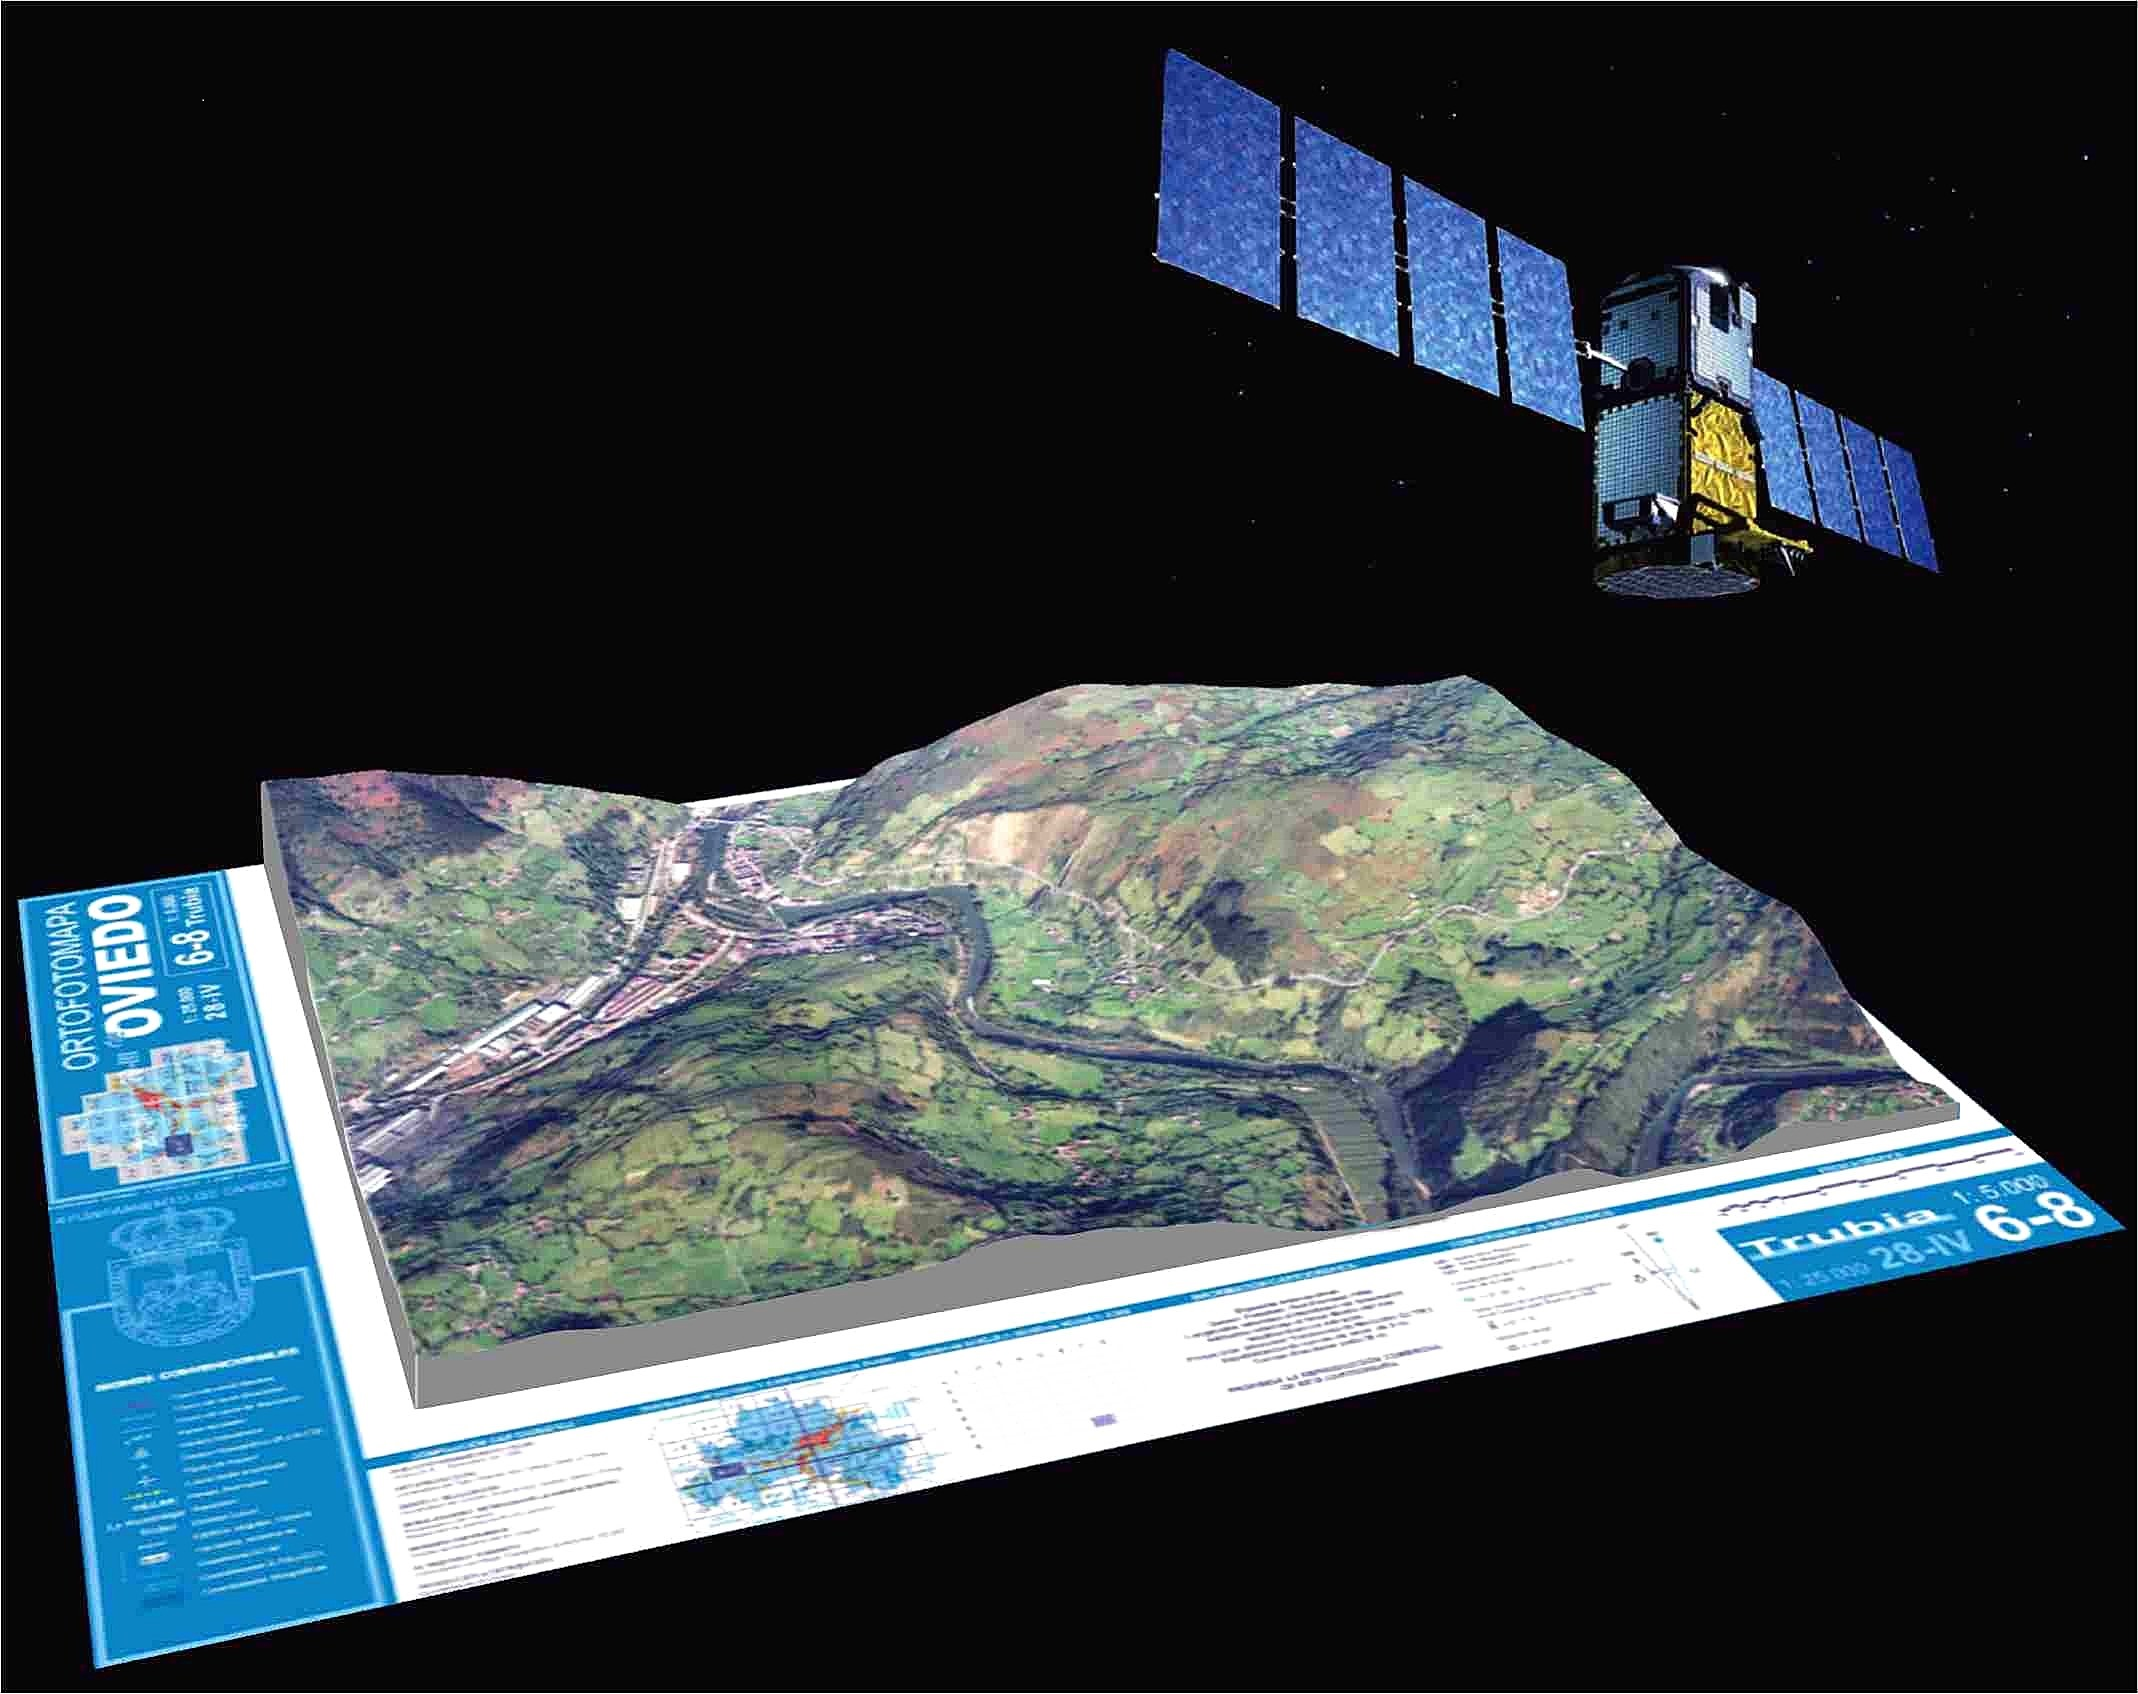
\includegraphics[width=\textwidth,height=1.875in]{int.jpg}

\begin{center}
{\large \textbf{Introducción a la Geomática}}\\

\end{center}
\justify

La Geomática es una ciencia que engloba las Geociencias (por ejemplo:
los sistemas de información geográfica (SIG)) con la integración y
aplicación de las tecnologias de la información y la comunicación (TICs)
Esta integración hace posible la captura, procesamiento, análisis,
interpretación, almacenamiento modelización, aplicación y difusión de
información digital geoespacial o localizada, aplicable en los ámbitos
de la ingenieria, el territorio y la sociedad.

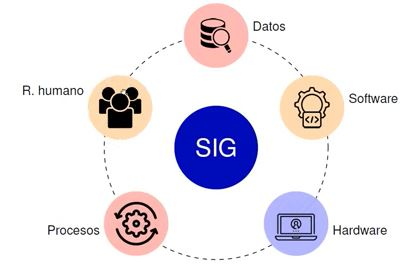
\includegraphics[width=\textwidth,height=2.29167in]{1.jpg}

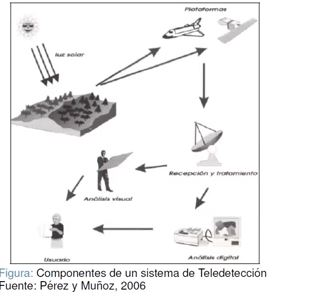
\includegraphics[width=\textwidth,height=3.33333in]{2.jpg}

El primer paso hacia la creación del dato geográfico implica el
establecimiento de un modelo conceptual relativo a cómo se ha de
interpretar la realidad geográfica. Se trata de conceptualizar el
espacio estudiado, la variable tratada y la variación de esta a lo largo
del espacio.

\textbf{Campos}

*Un campo es un modelo de variación dentro de un marco n-dimensional en
el cual en cada punto dentro de dicho masco se tiene un valor de la
variable estudiada

*La mayoria de las variables que se emplean en un SIG necesitan un único
valor para describirse (piensese en variables como la elevación, la
temperatura o la presión atmosérica, que solo requieren de un numero
para expresarse)

\textbf{Entidades discretas}

*No asocia a cada punto geográfico un valor, sino que concibe un entorno
geografico cono un espacia vacia sobre el que se sitúan distintos
elementos (entidades) que lo van menando

*Son en general más sencillas de comprender como concepto fuera de un
ámbito técnico

\textbf{Conceptualización}

Los modelos geográficos nos ofrecen una concepcion particular del
espacio geográfico y sus atributos. En base a ellos, el siguiente paso
es reducir las propiedades de dichos modelos a un conjunto finito de
elementos de tal modo que el registro de dichos elementos sirva para
almacenar la realidad que los modelos geográficos describen. Para ello,
empleamos los modelos de representación, también denominados modelos de
datos.

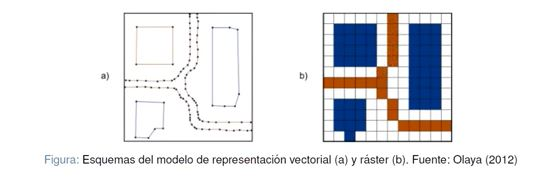
\includegraphics[width=\textwidth,height=1.875in]{3.jpg}

\textbf{Fundamentos}

Los modelos de representación definen una forma de recoger la realidad
mediante unidades básicas (sean estas celdas en una malla, o bien
primitivas geométricas definidas de una u otra manera), mientras que los
modelos de almacenamiento plantean básicamente un esquema de cómo
convertir dichas unidades en valores numéricos de la forma más
eficiente. Es decir, como escribir dichos valores en un soporte digital
o guardarlos en la memoria del ordenador de la mejor manera posible

\newpage
\begin{center}
{\large \textbf{Universidad Técnica de Machala}}\\
\textbf{Facultad de Ciencias Agropecuarias}\\
\textbf{Carrera de Agronomía}
\vspace{2mm}
\textbf{Geomática}
\end{center}

\begin{enumerate}
\def\labelenumi{\arabic{enumi}.}
\tightlist
\item
  \textbf{Datos Informativos}
\end{enumerate}

\textbf{Semana:} 2

\textbf{Fecha:} Pasaje, 02 de Junio 2022

\textbf{Fundamentación}

\textbf{objetivo}

\textbf{Procedimineto}

-Conectar directorio, primero crear carpeta dentro del disco duro, si
está fraccionado utilizar, la unidad \textbf{D},caso contrario utilizar
la unidad \textbf{C}

\textbf{Crear una carpeta: }

\emph{dir.create(``Geomatica'')}

-Instalar y llamar librerias

\begin{Shaded}
\begin{Highlighting}[]
\FunctionTok{library}\NormalTok{(pacman)}
\FunctionTok{p\_load}\NormalTok{(raster,sf,tidyverse,rgdal,printr)}
\end{Highlighting}
\end{Shaded}

\textbf{Cargar información}

\begin{Shaded}
\begin{Highlighting}[]
\NormalTok{pts }\OtherTok{\textless{}{-}} \FunctionTok{read.csv}\NormalTok{(}\StringTok{"D:/ERICK/5to semestre/Geo/semana2/DatosMuestreo.csv"}\NormalTok{) }\SpecialCharTok{\%\textgreater{}\%} \FunctionTok{as\_tibble}\NormalTok{()}
\FunctionTok{table}\NormalTok{(pts)}
\end{Highlighting}
\end{Shaded}

\begin{longtable}[]{@{}lllllr@{}}
\toprule
Id & x & y & Da & pH & Freq \\
\midrule
\endhead
QBP1 & 620699.228 & 9636159.72 & 1.8 & 7.5 & 1 \\
\bottomrule
\end{longtable}

\textbf{Pasar de tabla a dato espacial}

\begin{Shaded}
\begin{Highlighting}[]
\NormalTok{pts\_sf }\OtherTok{\textless{}{-}} \FunctionTok{st\_as\_sf}\NormalTok{(pts, }\AttributeTok{coords =} \FunctionTok{c}\NormalTok{(}\StringTok{"x"}\NormalTok{,}\StringTok{"y"}\NormalTok{), }\AttributeTok{crs =} \DecValTok{32717}\NormalTok{)}
\NormalTok{pts\_sp }\OtherTok{\textless{}{-}} \FunctionTok{as}\NormalTok{(pts\_sf, }\StringTok{\textquotesingle{}Spatial\textquotesingle{}}\NormalTok{)}
\FunctionTok{table}\NormalTok{(pts\_sf)}
\end{Highlighting}
\end{Shaded}

\begin{longtable}[]{@{}llllr@{}}
\toprule
Id & Da & pH & geometry & Freq \\
\midrule
\endhead
QBP1 & 1.8 & 7.5 & c(620699.228, 9636159.72) & 1 \\
\bottomrule
\end{longtable}

\begin{itemize}
\tightlist
\item
  TAMBIÉN SE PUEDE BAJAR DATOS DESDE LA WEB
\end{itemize}

\begin{Shaded}
\begin{Highlighting}[]
\NormalTok{ecu }\OtherTok{\textless{}{-}} \FunctionTok{getData}\NormalTok{(}\StringTok{"GADM"}\NormalTok{, }\AttributeTok{country =} \StringTok{"ECU"}\NormalTok{, }\AttributeTok{level =}  \DecValTok{0}\NormalTok{ )}
\FunctionTok{plot}\NormalTok{(ecu)}
\end{Highlighting}
\end{Shaded}


\includegraphics{semana_2_files/figure-latex/unnamed-chunk-5-1.pdf}

\end{document}
